\documentclass{article}
\usepackage[margin=1in]{geometry} % Set margins.
\usepackage{authblk} % Better formatting of affiliations.
\usepackage{url} % Allow URLs.
\usepackage{graphicx} % Allow figures.
\usepackage{xcolor} % Allow colored text.

\title{The Percolator 3.6 Mass spectrometry data post processor}

\author[1]{Lukas K\"{a}ll}
\author[2,3]{William Stafford Noble}
\author[4]{Will Fondrie}
\author[1]{Markus}
\author[5]{Matthew The}
\author[2]{Charles Grant}

\affil[1]{Science for Life Laboratory}
\affil[2]{Department of Genome Sciences, University of Washington}
\affil[3]{Paul G.\ Allen School of Computer Science and Engineering,
  University of Washington}
\affil[4]{Talus Biosciences}
\affil[5]{FIXME}

% For things that need to be fixed.
\newcommand{\fixme}[1]{\color{red}FIXME: #1\color{black}}

\begin{document}

\maketitle

\begin{abstract} 
This is a very abstract abstract.
\end{abstract}

\section{Introduction}

The Percolator algorithm, first described in 2007 \cite{kall:semi-supervised}, has become one of the most widely used software tools in the field of mass spectrometry proteomics.
The Percolator software takes as input database search results produced by any one of a variety of search tools and then applies a semi-supervised machine learning approach to rank the identified spectra based on the quality of the peptide-spectrum matches.

\section{Methods}

\section{Results}

\subsection{Speeding up Percolator}

We implemented two speedups in Percolator.
First, we incorporated a Windows-compatible version of conjugate
gradient least squares support vector machine training \cite{halloran:speeding}.
Second, we implemented a layer-ordered heaps sorting and selection
strategy for partitioning training sets \cite{lucke:performing}.

On an Intel-i5 9600K-3.7 GHz-6core cpu, we measure a performance increase of 84\% with the new code as compared to version 3.04 when processing a very large set of $3\cdot10^8$ peptide-spectrum matches.

% ==> 3-04-wilhelm-30M-psms.log <==
% real	179m2,265s
% user	494m24,008s
% ==> master-wilhelm-30M-psms.log <==
% real	97m12,910s
% user	234m34,415s

\begin{figure}
  \begin{center}
    \begin{tabular}{ccc}
    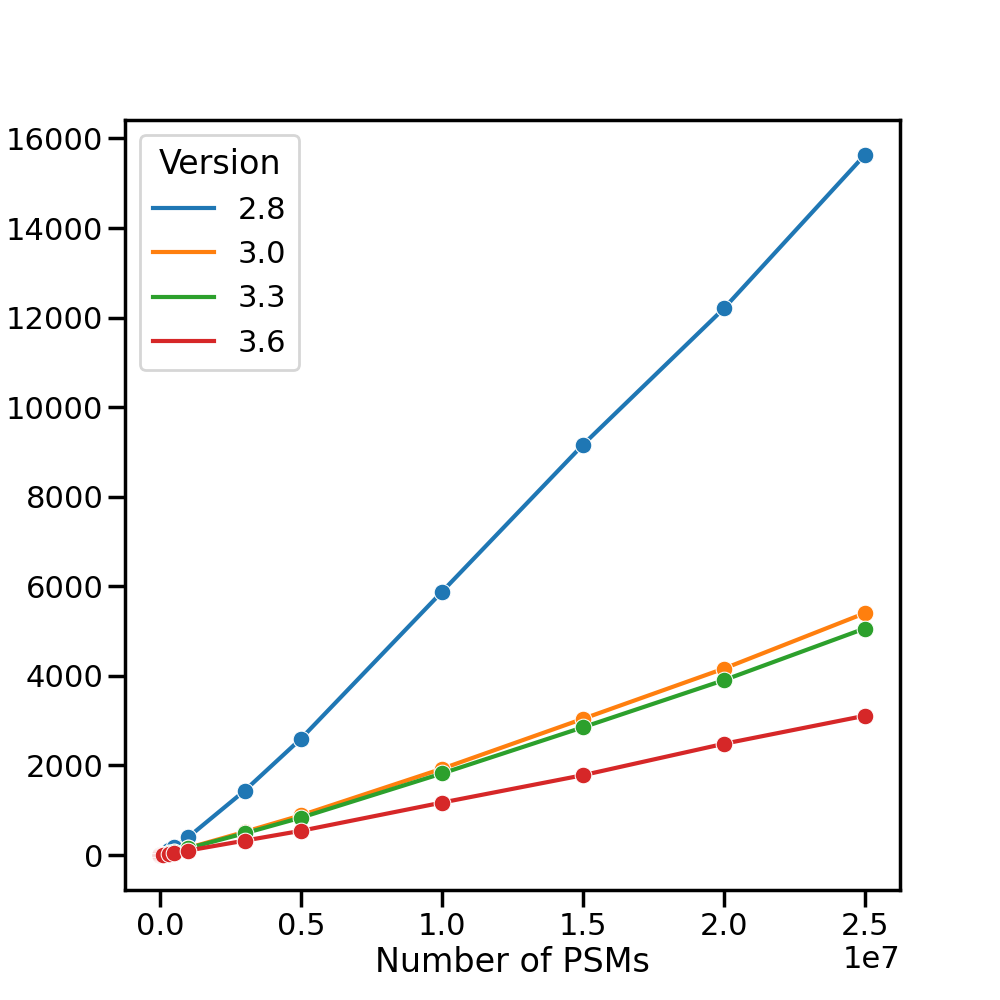
\includegraphics[width=0.3\linewidth]{img/wall.png} &
    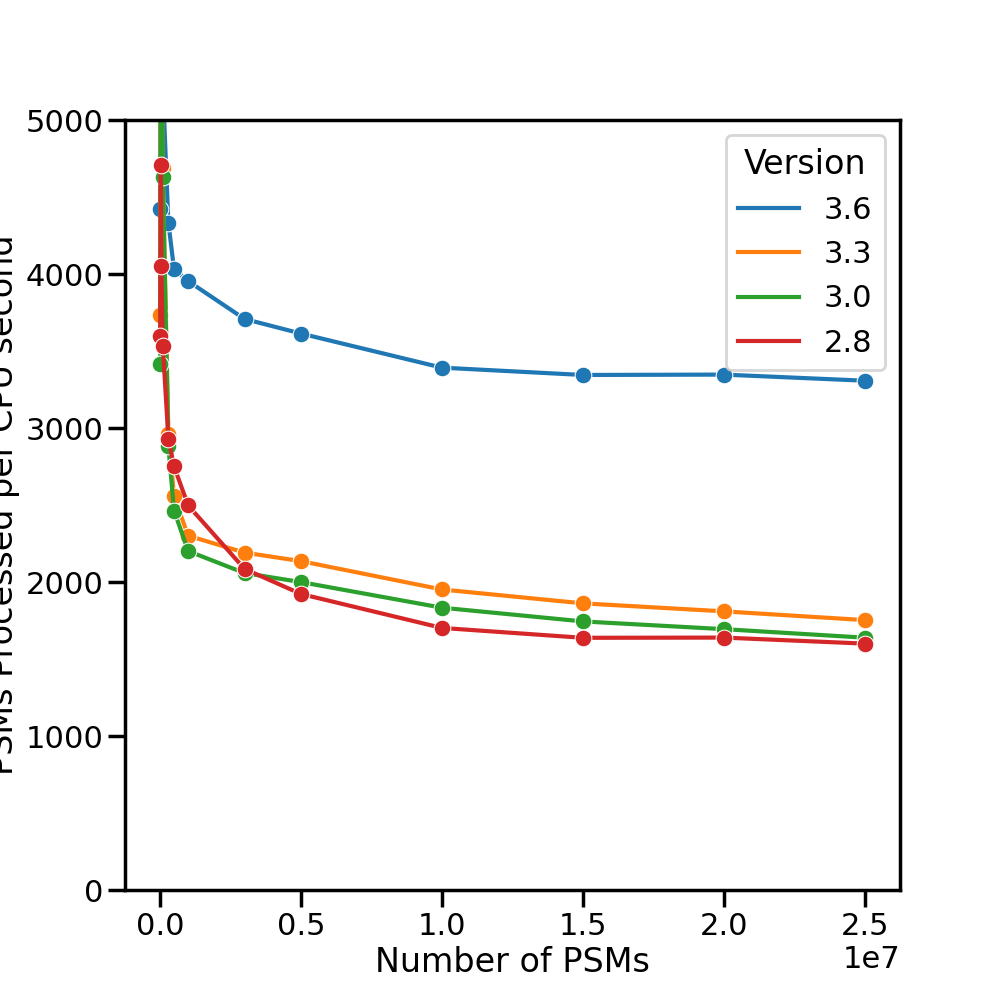
\includegraphics[width=0.3\linewidth]{img/rate.png} &
    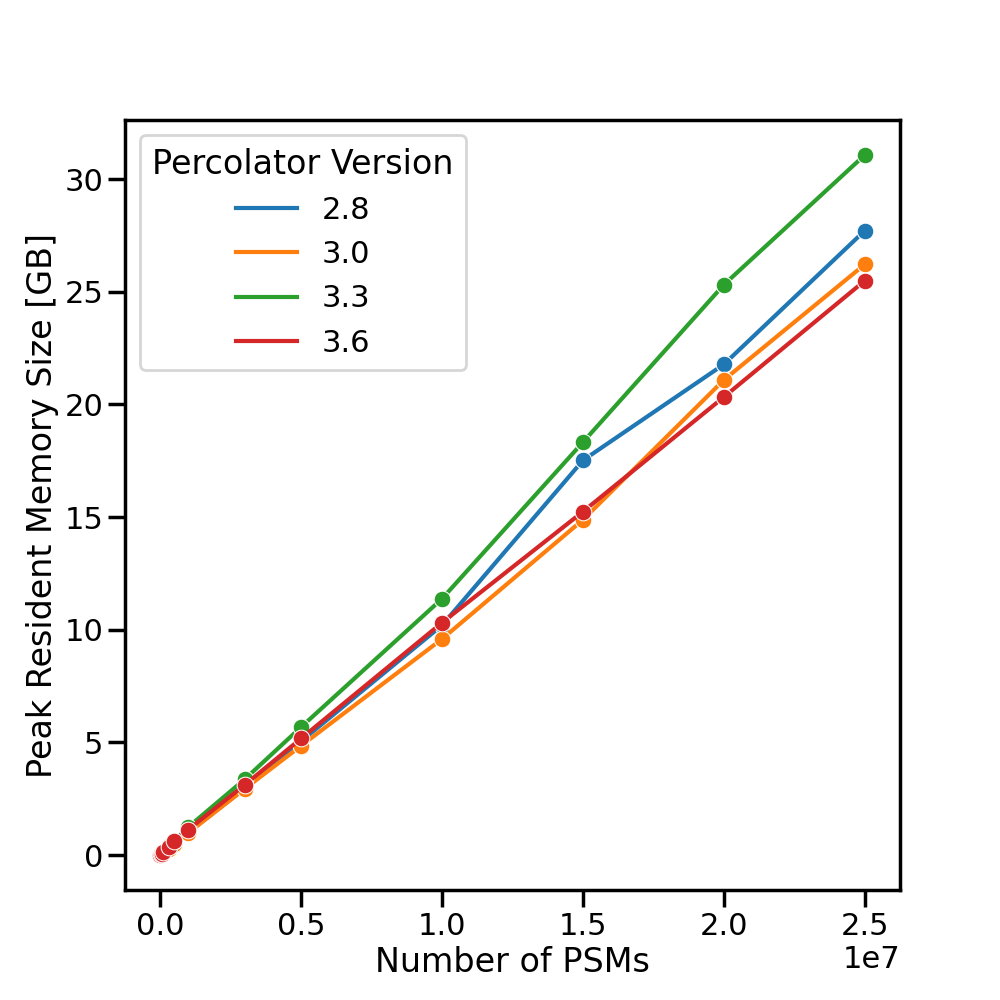
\includegraphics[width=0.3\linewidth]{img/memory.png} \\
    A & B & C \\
    \end{tabular}
    \caption{\textbf{Comparison of usage of resources between versions of Percolator} 
    (A) Wall time i.e. the actual time for the job to execute (B) The number of PSMs processed per CPU second 
    (C) The Peak Resident Memory Size, i.e. the amount of RAM needed.}
    \label{fig:x}
  \end{center}
\end{figure}

\subsection{Integration with FragPipe}

Benchmark between fragpipe with Peptide Prophet and with Percolator?

We have implemented a protocol for using Percolator to match MS1 precursors accross different mass spectrometry runs based on their difference in mass and retention time \cite{the:focus}, which allows the software to be used for label-free quantification.

We have also implemented an interface to the OpenSWATH module EasyPQ, thereby facilitating using Percolator as a part of data-independent acquisition
workflows.

\section*{Discussion}

Behind the scenes, we have also improved Percolator from a software engineering perspective.
First, we have implemented continuous integration of the Percolator source code via Github Actions.
This implementation automatically generates installation packages for Windows, MacOS, Ubuntu and CentOS.
Second, we have created extensive automated unit testing.
To do so, we have integrated the Google Test framework into the CMake build, as an optional feature.
The automated build system runs the unit test suite automatically with each check-in and includes support for the code coverage tool gcov.

\paragraph{Acknowledgements}

This work was supported by \fixme{get verbiage for CZI award.}

\bibliographystyle{plain}
\bibliography{percolator}

\end{document}
